\section{Classifiers Results and Discussion}

In this section, we present and analyze the results of the best candidate models obtained from both the traditional and \ac{dl}-based \ac{ser} approaches.

The top-performing model from the traditional approach is an \ac{xgb} classifier, utilizing 33 audio features as input. This model achieved an accuracy of 60.69\% after performing 5-fold \ac{cv} on the \ac{iemo} dataset. On the other hand, the final model obtained from the \ac{dl} approach is a Resnet50 model, which uses audio spectrogram images as input. This model achieved an accuracy of 58.24\% using the same evaluation strategy and dataset.


\subsection{Models Cross-Dataset Validation}

The performance of the final models trained using the \ac{iemo} dataset and tested on three different datasets, namely eNTERFACE'05, EMO-DB, and CREMA-D, are presented in Table \ref{final_models}. The cross-dataset validation was performed to evaluate the generalization capabilities, robustness, and significance of trained models. By testing the models on datasets with different recording conditions, language, and emotional expression variability, we can assess their ability to generalize to new, unseen data. This is an important step towards creating robust \ac{ser} models that can be applied in real-world scenarios where the training data may not perfectly match the test data.


\begin{table}[H]
	\centering
	\caption{Final models trained on \ac{iemo} and evaluated on different datasets.}
	\label{final_models}
	\resizebox{\textwidth}{!}{%
		\rowcolors{2}{gray!25}{white}
		\begin{tabular}{llrrrrrr}
			\toprule
			Dataset & Model & Accuracy & Macro F1 & Precision & Recall & \ac{mcc} & Time \\
			\midrule
			\addlinespace[1mm]
			
			eNTERFACE'05 & Traditional & 32.22 & 17.25 & 29.09 & 24.17 & 0.08 & 0.17 \\
			& \acl{dl} & 36.67 & 22.91 & 44.36 & 27.50 & 0.087 & 0.25 \\
			
			\midrulec
			\addlinespace[1mm]
			
			EMO-DB & Traditional & 38.35 & 15.82 & 14.80 & 26.06 & 0.07 & 0.10 \\
			& \acl{dl} & 38.35 & 15.79 & 37.78 & 25.99 & 0.066 & 0.18 \\ 
			
			\midrulec
			\addlinespace[1mm]
			
			CREMA-D & Traditional & 45.22 & 38.96 & 47.62 & 46.41 & 0.3151 & 0.10 \\
			& \acl{dl} & 54.14 & 47.71 & 51.68 & 52.98 & 0.407 & 0.30 \\
			
			
			\bottomrulec
		\end{tabular}%
	}
\end{table}


The \ac{dl} model generally outperformed the traditional model on all datasets, except for the EMO-DB dataset, where they performed similarly. The best overall performance was achieved on the CREMA-D dataset, with the \ac{dl} model achieving an accuracy of 54.14\% and a macro F1 score of 47.71\%.

However, both models exhibited poor results on the eNTERFACE'05 and EMO-DB datasets, with accuracy scores of less than 40\%, and, in terms of macro f1-scores they are slightly better for the eNTERFACE'05 but still low. A low macro F1 score means that the model's ability to correctly classify instances of different classes is poor. This could be due to several factors, such as class imbalance or the model's inability to capture important features that distinguish between different classes.

In terms of computation time, the traditional models were faster than the \ac{dl} models, which is evident from the lower time values in the table. This is a crucial factor when employing these models for real-time emotion recognition systems.

Further insights into the obtained results can be obtained through the confusion matrices, as shown in Figure \ref{fig:final_cm}. We can observe both models predicted the anger emotion multiple times across all three datasets. In the case of the eNTERFACE'05 dataset, which lacks neutral emotions, the \ac{dl} model predicted the happiness emotion more frequently compared to the traditional model, which is the leading reason for the slightly better results.

Analyzing the confusion matrix of the EMO-DB dataset, it is clear that the anger emotion was predicted for the majority of audio files, which is likely due to the German language used in the dataset known for its assertiveness and directness. However, this should not be interpreted as a flaw in the model's performance but rather a reflection of the language's characteristics used in the training and testing datasets. This highlights the English language bias of our \ac{ser} models and suggests that the results for other languages may not be satisfactory.

Moreover, the traditional model had difficulty recognizing the happiness emotion in the CREMA-D dataset, as in the eNTERFACE'05 dataset, and often confused the neutral emotion with sadness. Although the \ac{dl} model exhibited the same confusion, it predicted the sadness emotion more often.

Finally, it is worth noting that the traditional models were faster than the \ac{dl} models, with lower time values in the table, which is critical when implementing these models for real-time \ac{ser} systems.

In conclusion, the results suggest that the \ac{dl} model may be more suitable for the \ac{ser} task on diverse datasets, owing to its improved feature extraction and generalization abilities. However, the \ac{dl} model is slower compared to the traditional models, which can significantly impact real-time applications. Furthermore, we recommend that these models should be utilized for English-spoken audio recordings and preferably with less prominent accents, to minimize any language bias-induced errors.


\begin{figure}
	\begin{subfigure}{.5\textwidth}
		\centering
		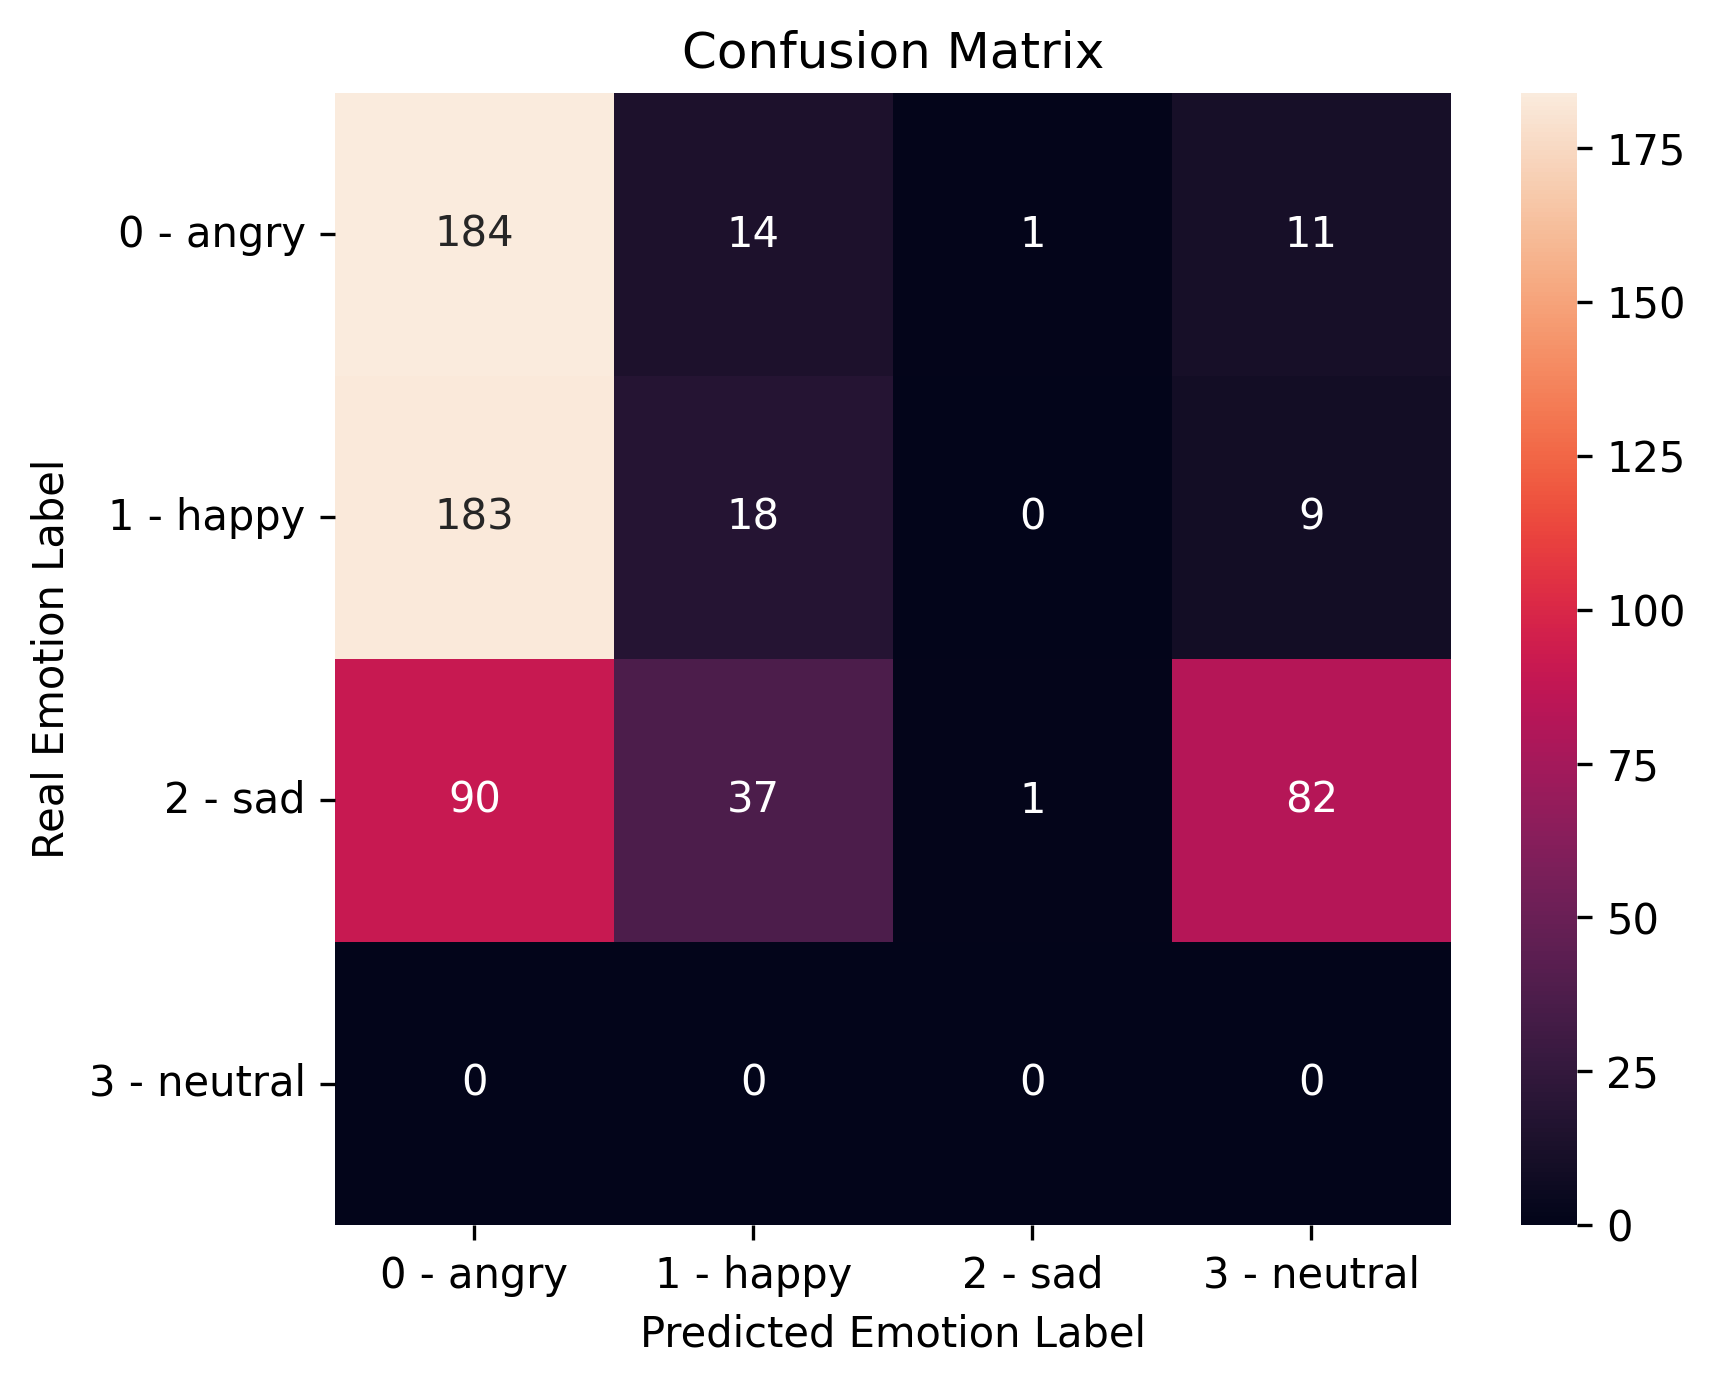
\includegraphics[width=\linewidth]{figs/4_5_discussion/ent_trad_cm.png}
		\caption{eNTERFACE'05 traditional model confusion matrix.}
	\end{subfigure}%
	\begin{subfigure}{.5\textwidth}
		\centering
		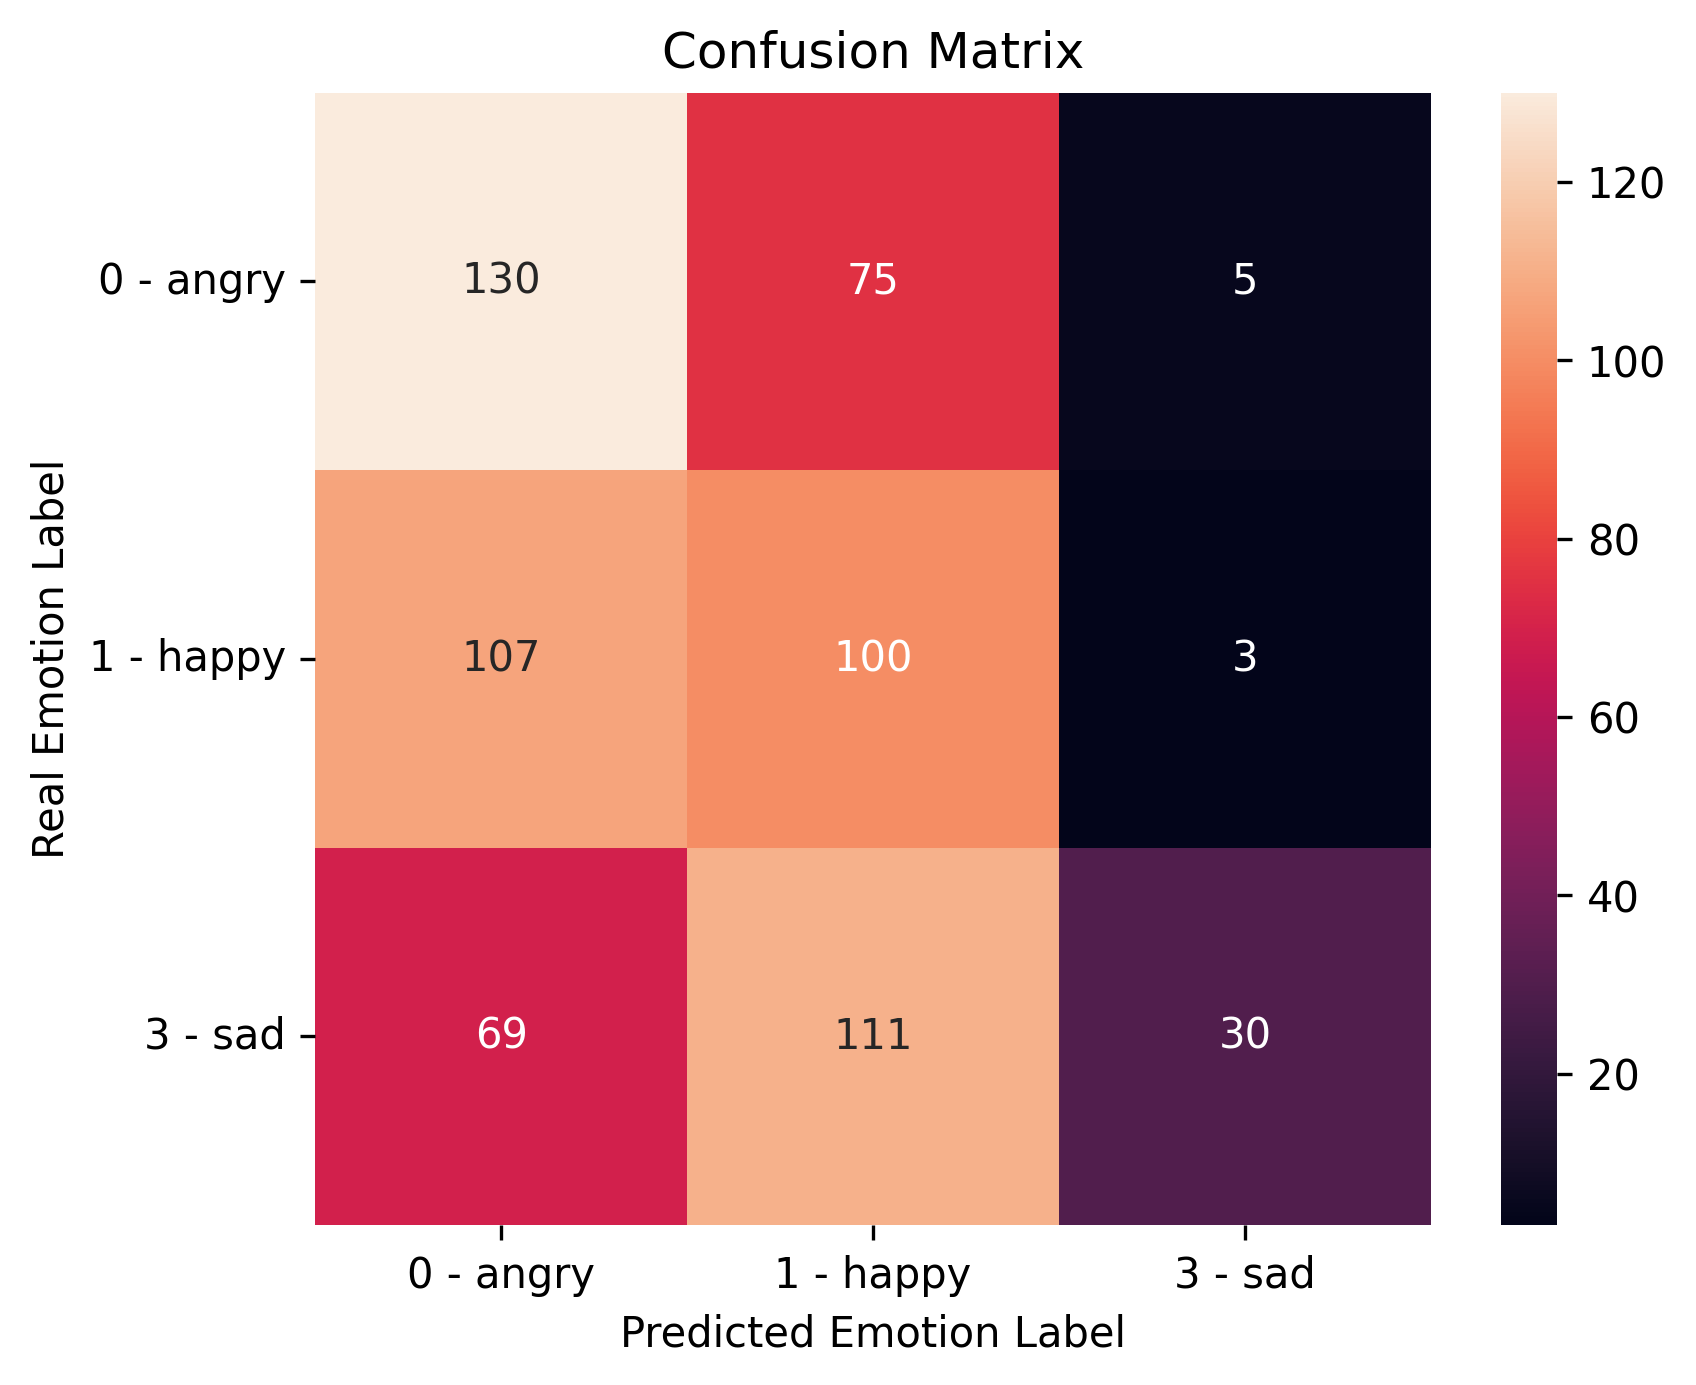
\includegraphics[width=\linewidth]{figs/4_5_discussion/ent_deep_cm.png}
		\caption{eNTERFACE'05 \ac{dl} model confusion matrix.}
	\end{subfigure}
	\newline
	\begin{subfigure}{.5\textwidth}
		\centering
		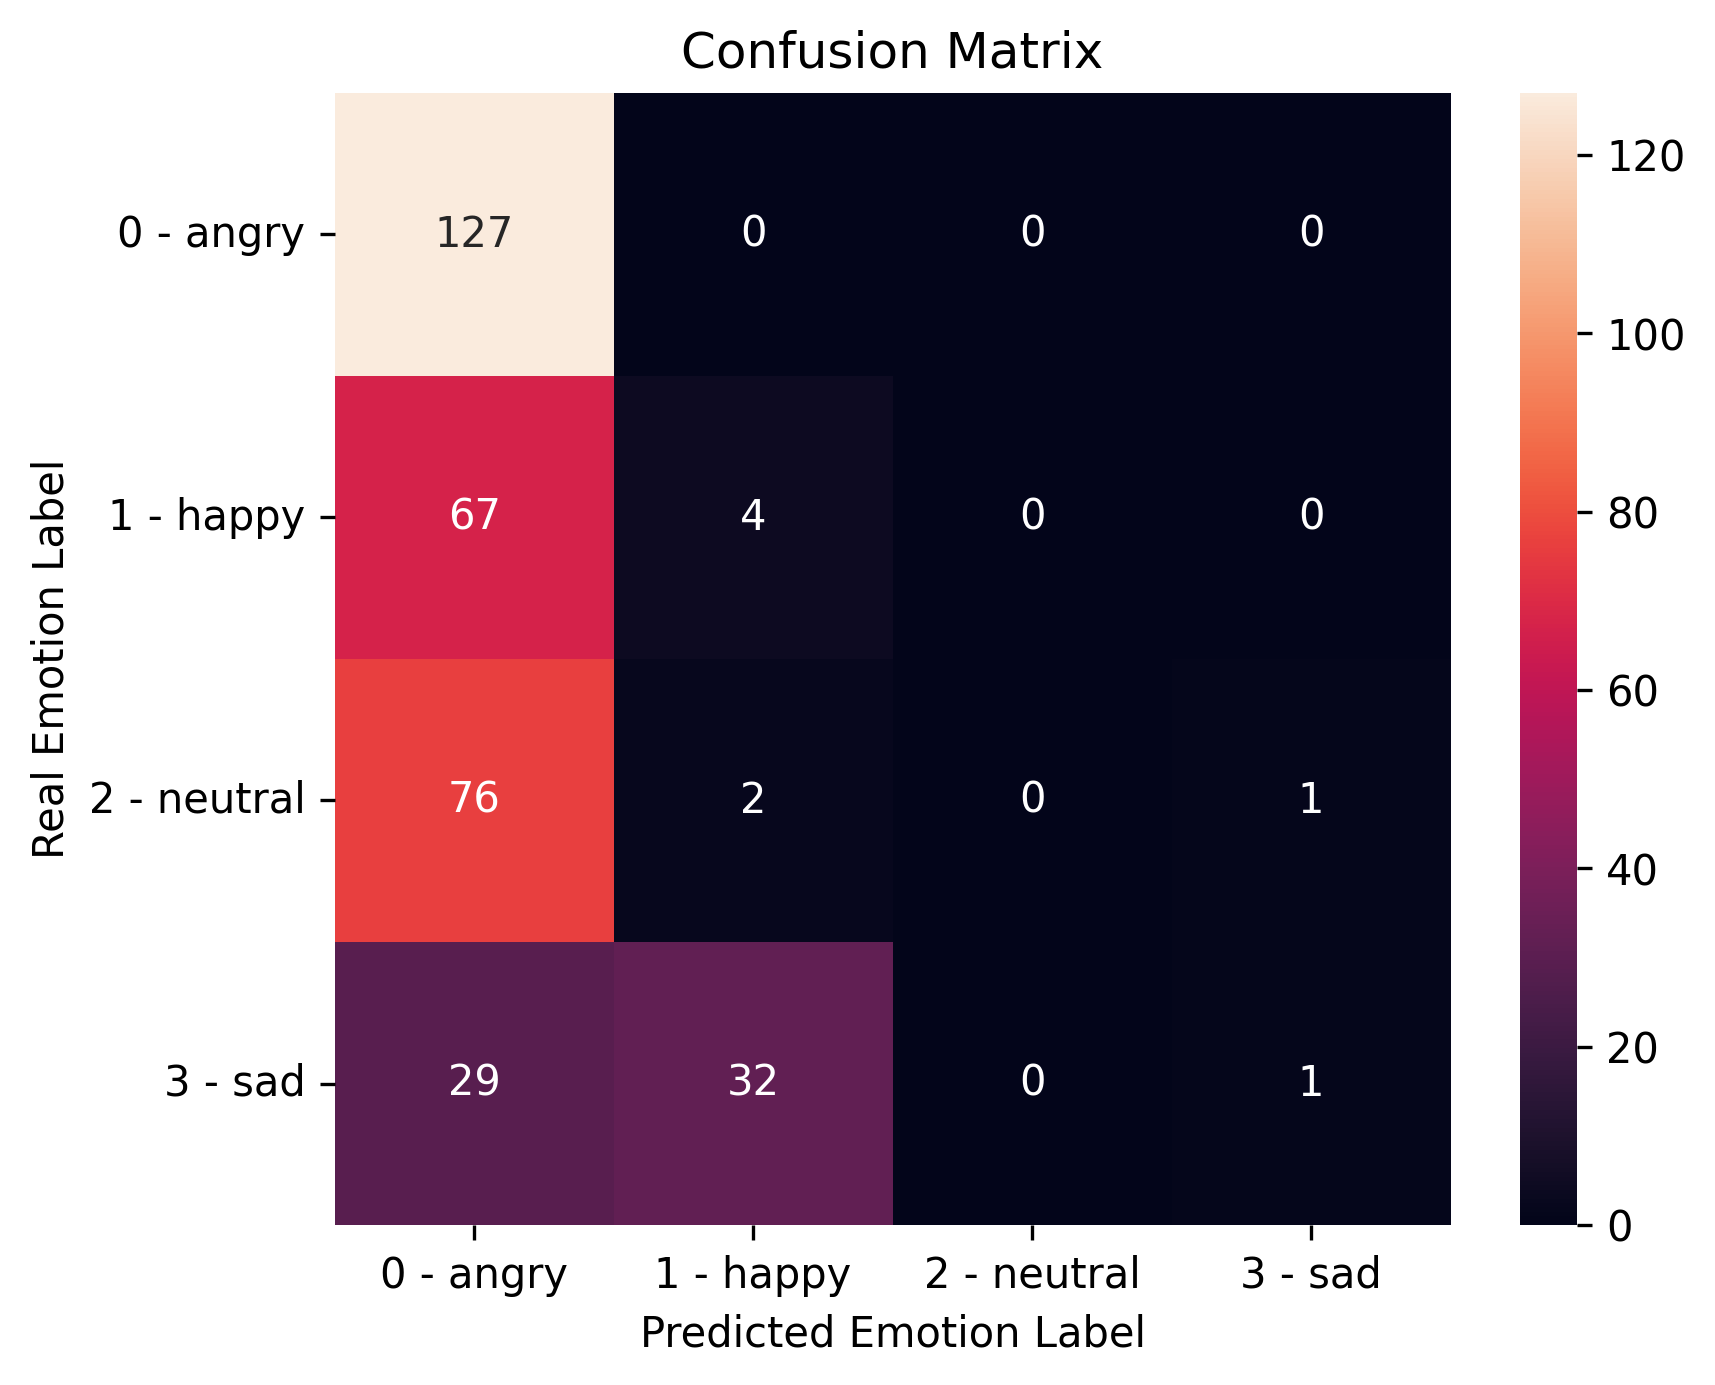
\includegraphics[width=\linewidth]{figs/4_5_discussion/emo_trad_cm.png}
		\caption{EMO-DB Traditional model confusion matrix.}
	\end{subfigure}%
	\begin{subfigure}{.5\textwidth}
		\centering
		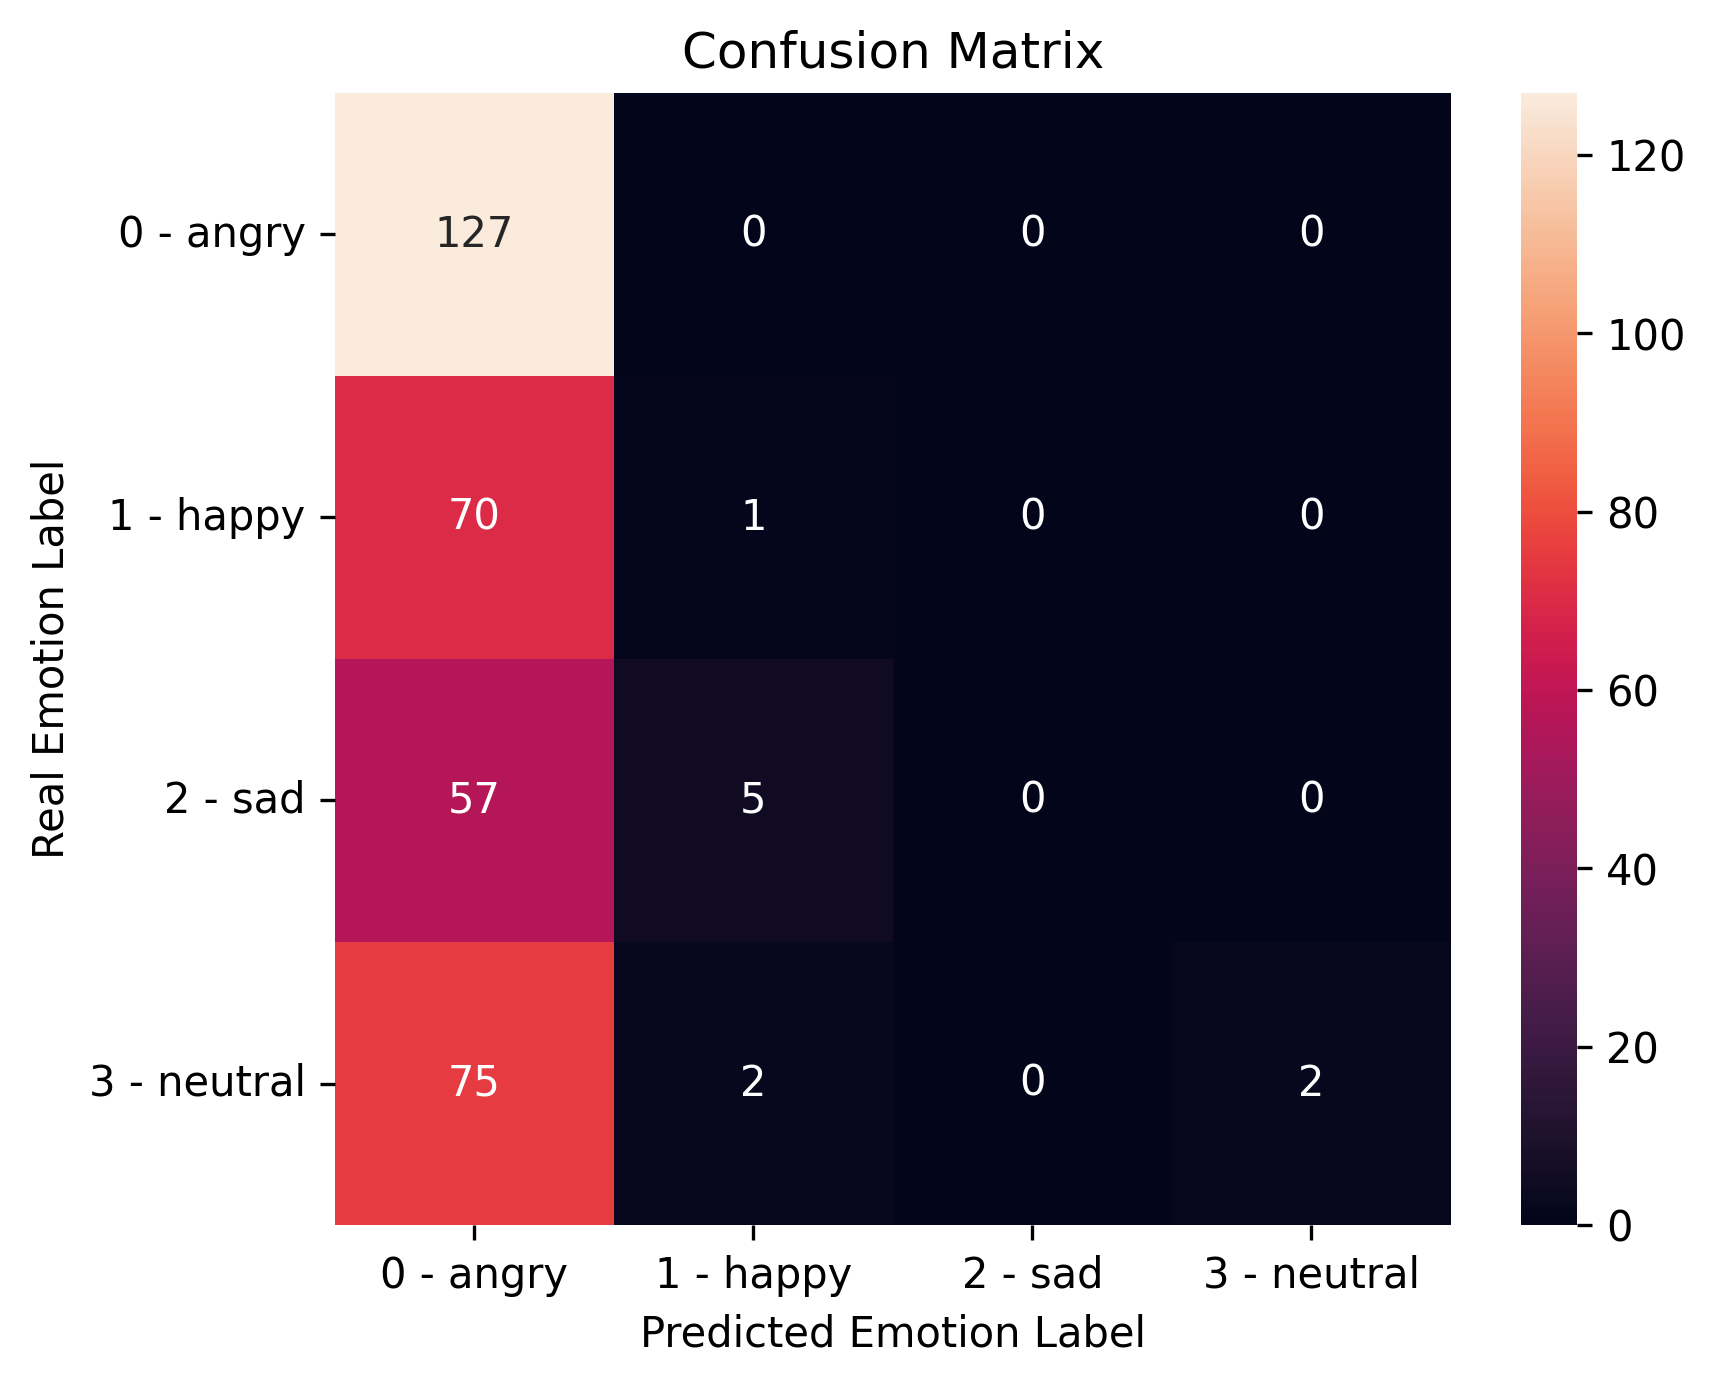
\includegraphics[width=\linewidth]{figs/4_5_discussion/emo_deep_cm.png}
		\caption{EMO-DB \ac{dl} model confusion matrix.}
	\end{subfigure}
	\newline
	\begin{subfigure}{.5\textwidth}
		\centering
		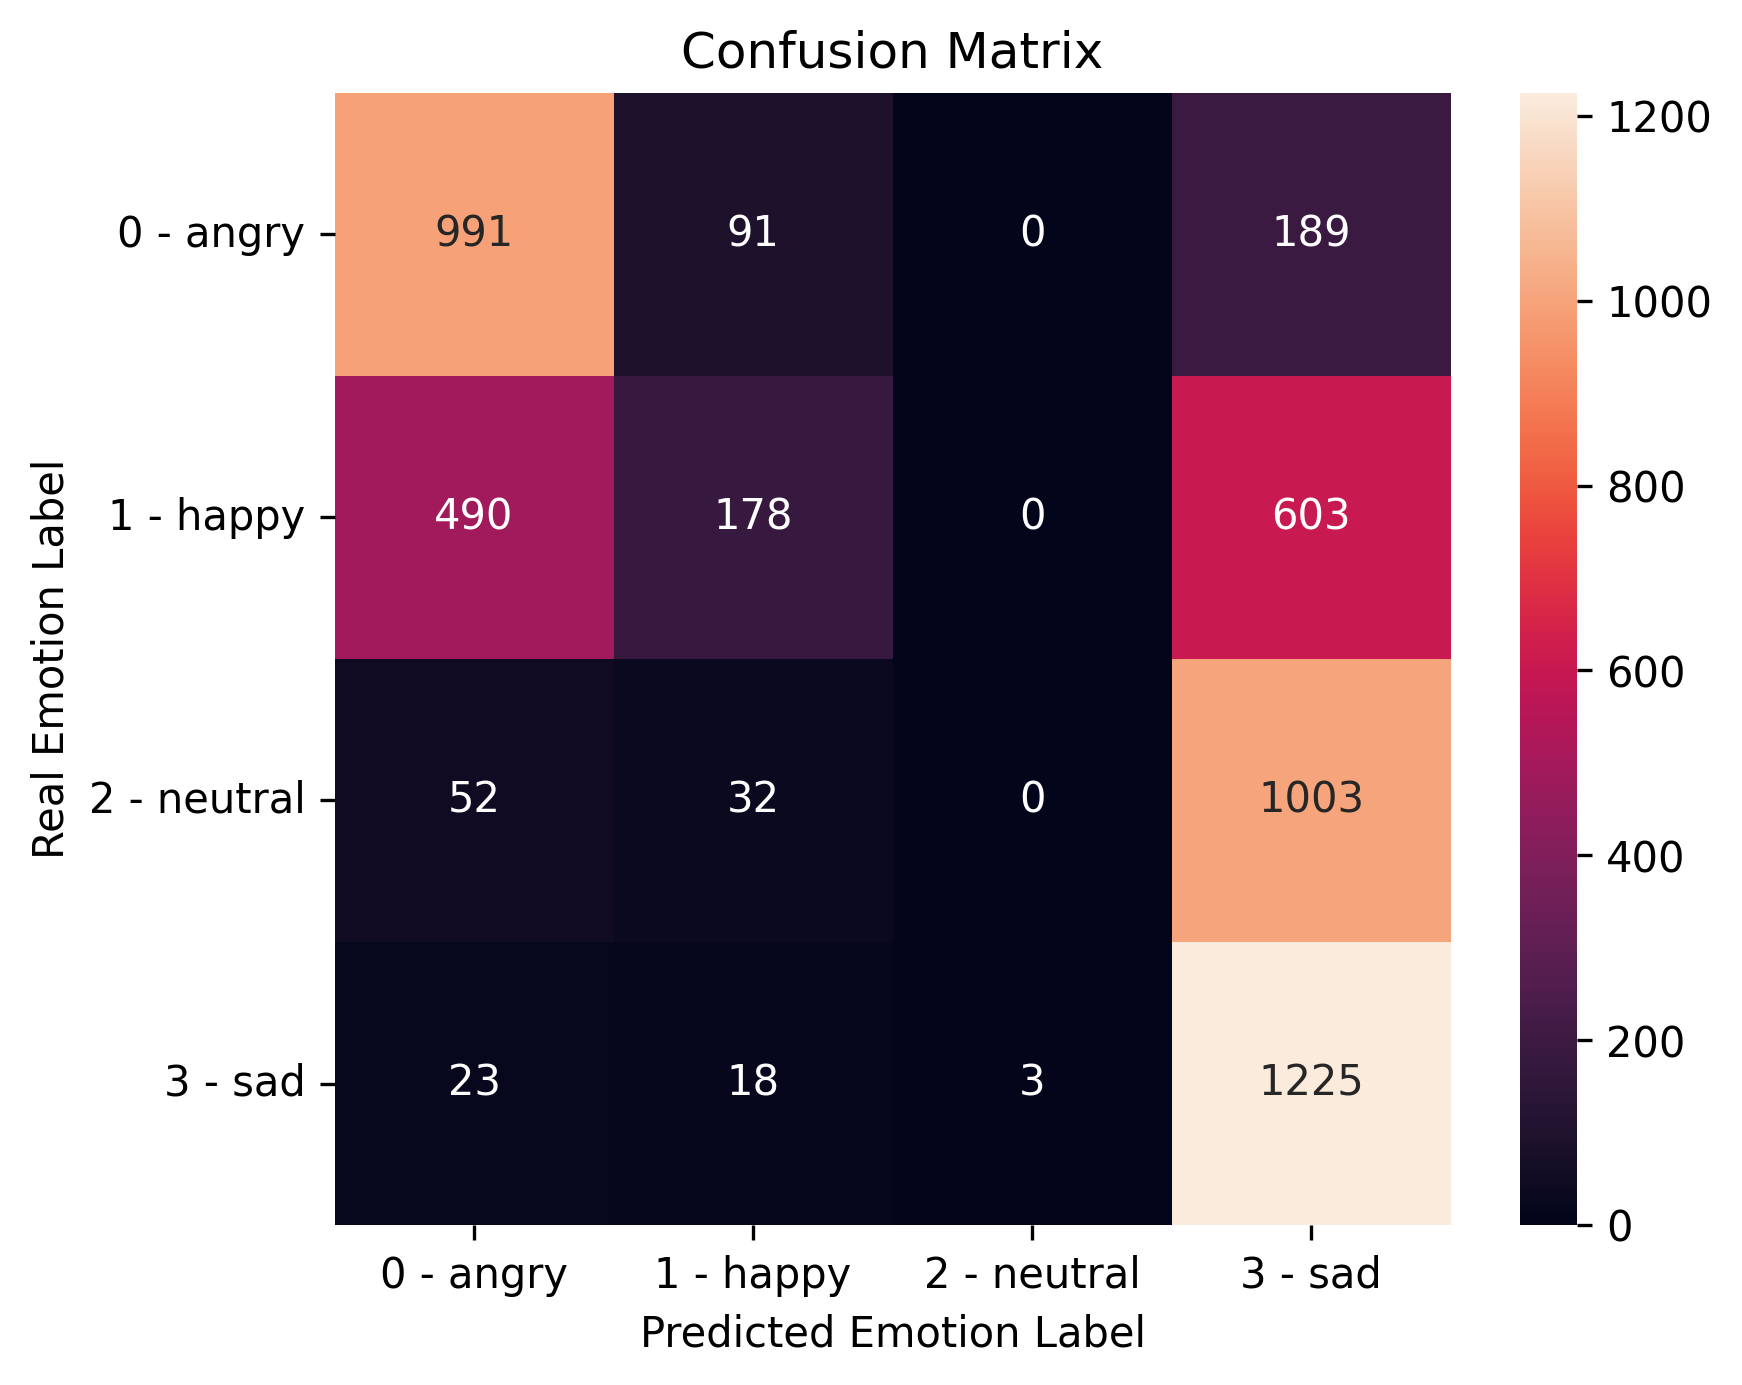
\includegraphics[width=\linewidth]{figs/4_5_discussion/cre_trad_cm.png}
		\caption{CREMA-D Traditional model confusion matrix.}
	\end{subfigure}%
	\begin{subfigure}{.5\textwidth}
		\centering
		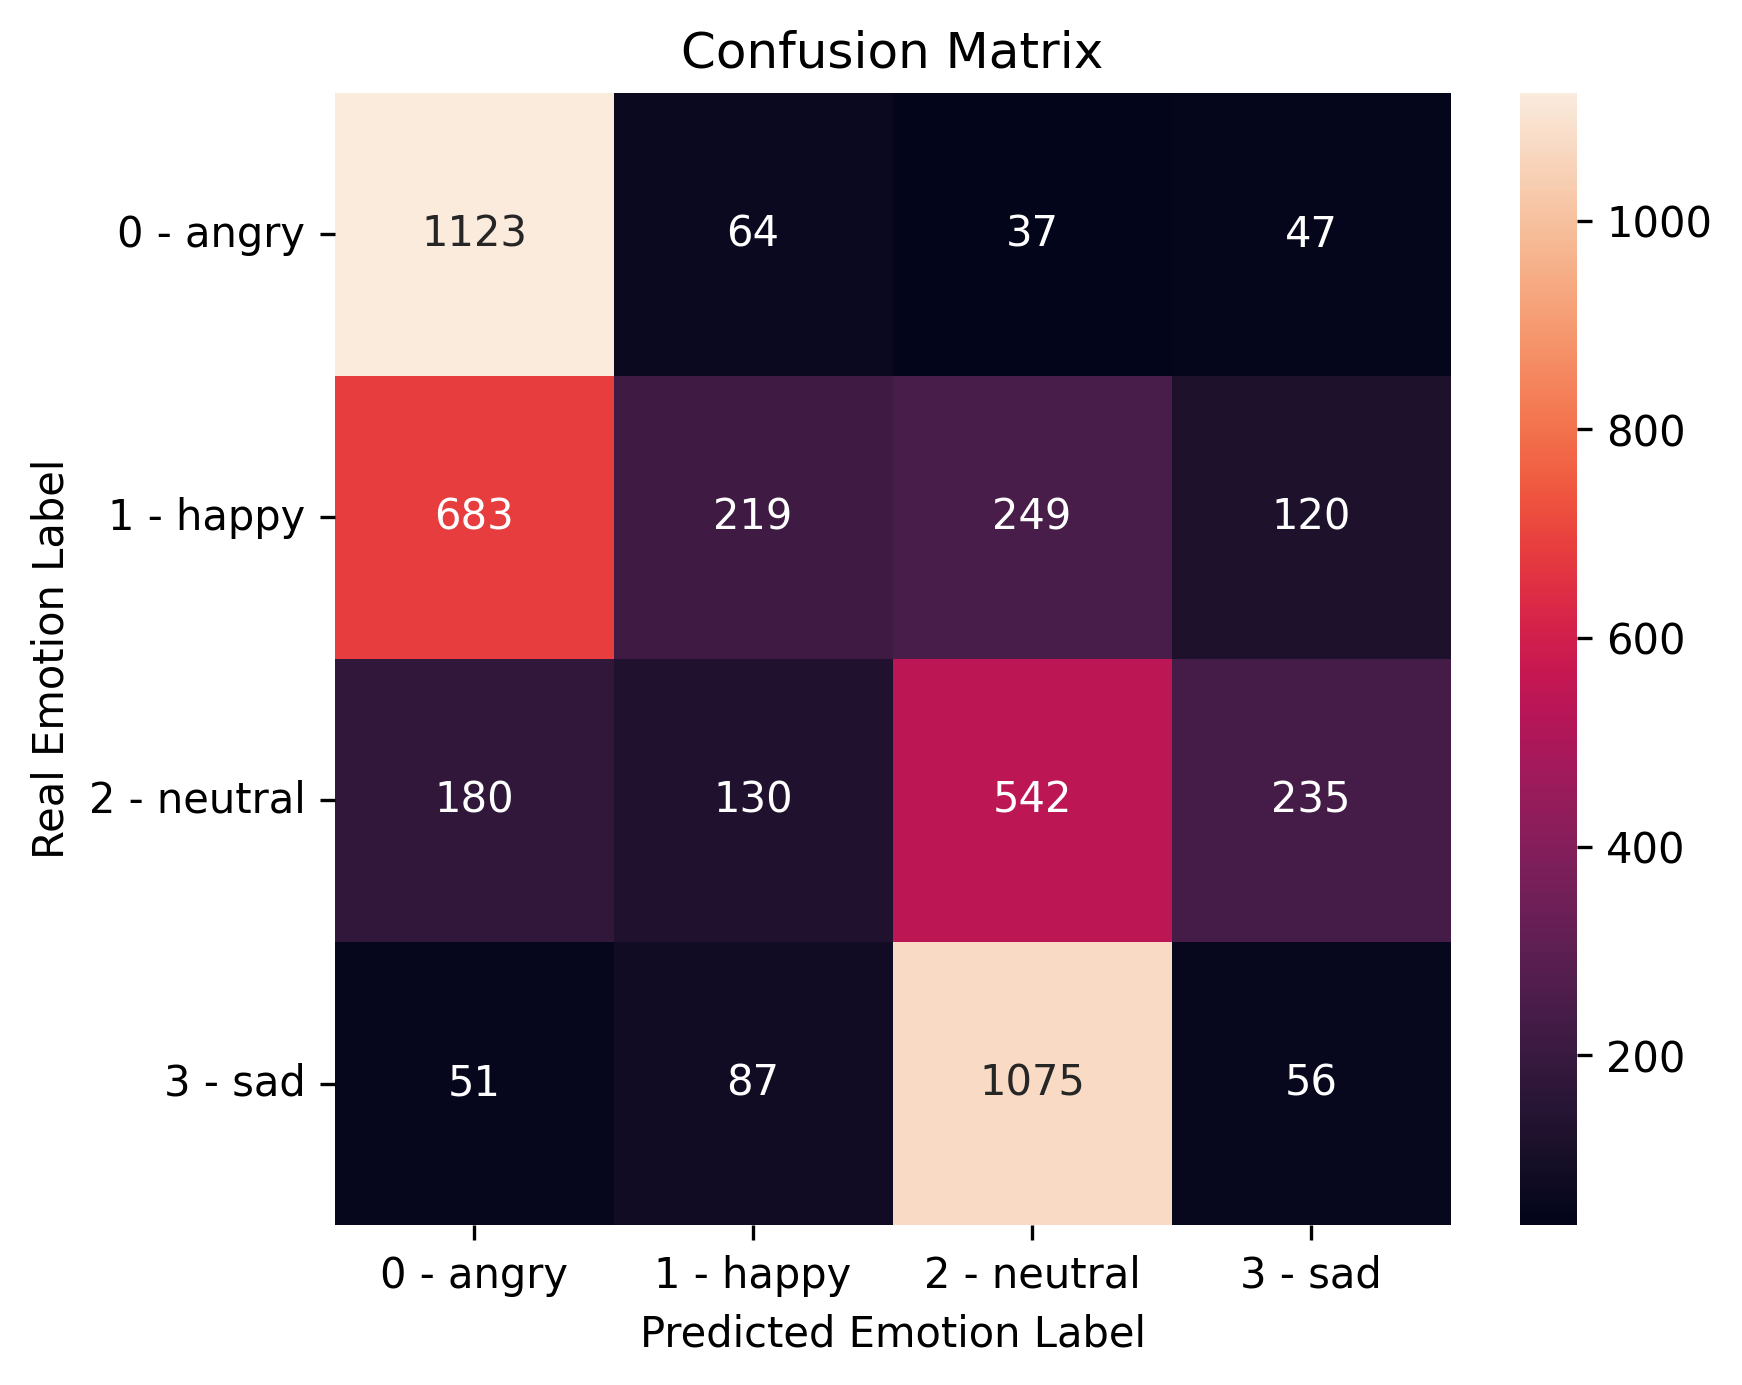
\includegraphics[width=\linewidth]{figs/4_5_discussion/cre_deep_cm.png}
		\caption{CREMA-D \ac{dl} model confusion matrix.}
	\end{subfigure}
	\caption{Final models confusion matrices on the eNTERFACE'05, EMO-DB and CREMA-D datasets.}
	\label{fig:final_cm}
\end{figure}


\subsection{\ac{sota} Comparison}

In Table \ref{tab:modelssoa}, we summarize the performance of various classification models on the \ac{iemo} dataset, including our proposed model (highlighted in blue). The first four rows represent traditional feature-based approaches, while the remaining rows represent \ac{dl}-based approaches.

It is important to note that the \ac{sota} results are not always directly comparable, as different authors may use different subsets of data and evaluation methodologies. For instance, some authors may not consider the emotion of excitement as happiness, others may only use improvised data and not scripted, or even perform different validation methods such as 10-fold \ac{cv}. Additionally, the random seeds for the k-fold splits may also impact the final classification performance.

Our proposed model, an \ac{xgb} classifier utilizing 33 audio features, achieved an accuracy of 60.69\% on 5-fold \ac{cv}, outperforming the traditional approaches presented in the first three rows. Another model from the traditional approach, that outperformed ours, utilized a \ac{cnn} for its feature extraction capabilities; however, we still consider it traditional as the authors still performed feature extraction to obtain the 193-dimensional feature vector for the model's input.

Among the \ac{dl}-based approaches, our Resnet50 model achieved an accuracy of 58.24\%, which is lower than the other \ac{sota} results. The Quaternion \ac{cnn} achieved the highest accuracy of 70.46\%, utilizing a unique approach of encoding the Mel spectrogram in an RGB quaternion domain, which may have contributed to its higher accuracy.

\begin{table}[H]
	\centering
	\caption{\ac{sota} \ac{ser} classification models performance on \ac{iemo}.}
	\label{tab:modelssoa}
	\resizebox{\textwidth}{!}{%
		\begin{tabular}{lccr}
			\toprule
			Model                      & Input & Evaluation Strategy & Accuracy (\%) \\
			\toprulec
			\rowcolor{gray!25}
			\multicolumn{4}{c}{Traditional Feature-Based \ac{ser} Approaches} \\
			\midrulec
			
			\begin{tabular}[l]{@{}l@{}}Ensemble of \ac{rf}, \ac{xgb}\\and Multilayer Perceptron\end{tabular} \cite{HandCraftedSahu} & \begin{tabular}[c]{@{}c@{}}8-dimensional audio\\features vector\end{tabular} & \begin{tabular}[c]{@{}c@{}}1 random 80:20\\train-test split\end{tabular} & 56.00 \\
			\addlinespace[1mm]
			
			\begin{tabular}[l]{@{}l@{}}Multi-level binary\\decision trees \cite{Lee2011}\end{tabular} & 384 audio features vector & 10 fold \ac{cv} & 58.46 \\
			\addlinespace[1mm]
			
			\rowcolor{LightCornflowerBlue}
			\ac{xgb} [Ours] & 33 audio features vector & 5-fold \ac{cv} & 60.69 \\
			\addlinespace[1mm]
			
			\ac{cnn} \cite{Issa2020}  & 193 audio features vector & 5-fold \ac{cv} & 64.30 \\
			\addlinespace[1mm]
			
			\toprulec
			\rowcolor{gray!25}
			\multicolumn{4}{c}{\acl{dl}-Based \ac{ser} Approaches} \\
			\midrulecb
			
			\rowcolor{LightCornflowerBlue}
			Resnet50 [Ours] & 3-D Spectrogram Image & 5-fold \ac{cv} & 58.24 \\
			\addlinespace[1mm]
			
			\ac{cnn} and \ac{rnn} \cite{ma18b_interspeech} & Log-Spectrogram & 5-fold \ac{cv} & 64.22 \\
			\addlinespace[1mm]
			
			\begin{tabular}[l]{@{}l@{}}3-D attention-based\\convolutional \ac{rnn} \cite{8421023}\end{tabular} & 3-D Mel-Spectrogram Image & 10-fold \ac{cv} & 64.7 \\
			\addlinespace[1mm]
			
			\begin{tabular}[l]{@{}l@{}}\ac{cnn} and \ac{lstm}\\with attention \cite{Zhao2019}\end{tabular} & Mel-Spectrogram & 5-fold \ac{cv} & 67.0 \\
			\addlinespace[1mm]
			
			Quaternion \ac{cnn} \cite{Muppidi2021} & \begin{tabular}[c]{@{}c@{}}Mel spectrogram\\ encoded in an RGB\\quaternion domain\end{tabular} & 5-fold \ac{cv} & 70.46 \\
			\addlinespace[1mm]
			
			\bottomrule
		\end{tabular}%
	}
\end{table}

\subsection{Discussion}

Our findings support the idea that the \ac{dl} model is better suited for \ac{ser} tasks on diverse datasets, due to its improved feature extraction and generalization capabilities of data under different factors. We believe this is mainly because the traditional approach relies on a feature input vector derived from the training dataset, limiting its applicability to other datasets. However, the traditional model is more suitable for real-time applications as it has a faster processing speed than the \ac{dl} model.

It is worth noting that our \ac{xgb} model achieved competitive results compared to the \ac{sota} approaches presented in the table, despite using only a 1-dimensional 33 audio feature vector. This makes it more computationally efficient than other traditional approaches that require a much larger number of features. Nonetheless, both of our models still have the potential for improvement, especially in the \ac{dl} approach where fine-tuning was limited due to its computational expense. We also recommend using our models for English-spoken audio recordings with less prominent accents to mitigate language bias since the training dataset contains English audio.

Overall, this chapter offers a comprehensive implementation and thought process, along with conclusions and interpretations of the obtained results, laying a solid foundation for future research in developing more robust and accurate \ac{ser} models. It highlights the importance of considering the impact of different validation methodologies used in \ac{ser} research to ensure the models' robustness and applicability to diverse datasets. These findings contribute to the growing body of research on \ac{ser} and provide valuable insights for researchers and practitioners in the field.
